
\documentclass[11pt, oneside]{article}   	% use "amsart" instead of "article" for AMSLaTeX format
\usepackage{geometry}                		% See geometry.pdf to learn the layout options. There are lots.
\usepackage{animate}
\geometry{letterpaper}                   		% ... or a4paper or a5paper or ... 
%\geometry{landscape}                		% Activate for rotated page geometry
%\usepackage[parfill]{parskip}    		% Activate to begin paragraphs with an empty line rather than an indent
\usepackage{graphicx}				% Use pdf, png, jpg, or eps§ with pdflatex; use eps in DVI mode
								% TeX will automatically convert eps --> pdf in pdflatex		
\usepackage{amssymb}

%SetFonts

%SetFonts


\title{Quasicrystal Scattering and the Riemann Zeta Function}
\author{Michael Shaughnessy}
%\date{}							% Activate to display a given date or no date

\begin{document}
\maketitle

\begin{abstract}
I carry out scattering calculations against a one-dimensional point like arrangement of atoms, $\mathbf{\chi(x)}$, related to the distribution of prime numbers by a shift operation making the atomic density approximately constant. 
I show how the Riemann Zeta Function (RZF) naturally parameterizes the analytic structure of the scattering amplitude. 
Inspired by Dyson's quasicrystal suggestion \ref{Dyson} I present a cryptic speculation in the Appendix, vaguely indicating how the real component of every non-trivial zero of the storied Riemann Zeta Function might be determined.
\end{abstract}

\section{Introduction}

There have been many explanations of the curious relationship between the prime numbers and the values of the non-trivial zeros of the Riemann Zeta Function (RZF).

\ref{Riemann, Selberg, Dyson, Zhang}

Freeman Dyson \ref{Baez} speculated about a possible path to determining the relationship between the real and the imaginary components of the non-trivial zeros of the RZF, using the concept of a quasicrystal.

A quasiperiodic crystal, or quasicrystal, is a structure that is ordered but not periodic.

Quasicrystals were experimentally observed by Shechtman in 1985 \ref{Shechtman1985}. 

B. Riemann showed the prime numbers are partially ordered and are not periodic \ref{Riemann1859} in 1859 and H. Von Mangoldt \ref{VonMangoldt1895} proved the explicit formula in 1895.

The explicit formula of Guinand and Weil \ref{Weil} is a formula for the Fourier transform of the RZF zeros as a sum over prime powers, plus additional terms.  


%\subsection{Fourier Transform}
%\begin{figure}
 %   \centering
%    \animategraphics[width=0.8\linewidth,autoplay,loop]{627}{../animations/FT_animation-}{0}{626}
%    \caption{Fourier Transform animated. Open with Adobe Acrobat Reader to watch}
%    \label{fig:FT_animation}
%!TEX encoding = UTF-8 Unicode\end{figure}

The Fourier transform of $V(x)$ is $\hat{V}(k)$ 

\begin{equation}
\hat{V}(k) = \int_{-\infty}^{\infty}V(x)e^{-i2\pi kx}dx
\end{equation}

A one-dimensional scattering potential may be of the form 
\begin{equation}
V(x) = \sum_{x_n \in X}\delta_D(x - x_n)
\end{equation} 
 
where the $x_n$ are elements of a countable set of real numbers. 
Then $V(x)$ is called a tempered distribution.
 For certain $V(x)$ of the form above it is the case that it's Fourier transform, $\hat{V}(k)$, also contains a tempered distribution. 
  
\begin{equation}
 \label{eq: RiemannFourier}
 \mathcal{F}\left \{V(x)\right \} = \hat{V}(k) = \mathcal{F}\left \{ \sum_{x_n \in X}\delta_D(x - x_n) \right \} = \hat{h}(k) +  \sum_{k_m \in X^{*}} \hat{V_{m}} \delta_D(k - k_{m}),
\end{equation}

If $\hat{h}(k) = 0$ everywhere, then $V(x)$ is called a quasicrystal.
By applying the Fourier transform a second time to $\hat{V}(k)$, it is evident that $\hat{V}(k)$ is also a quasicrystal when $V(x)$ is a quasicrystal. When all the $x_n$ lie along a line, the $k_m$ must also lie along a line in the complex plane - applying the Fourier transform twice gives us back our original $V(x)$.






%In general, $\hat{V}(k) =\hat{g}(k) + \hat{h}(k)$ may have a discrete component, $\hat{g}(k)$  and a continuous component, $\hat{h}(k)$.

%\begin{equation}
 %\label{eq: RiemannFourier}
 %\mathcal{F}\left \{ \sum_{x_n \in X}\delta_D(x - x_n) \right \} = h(k) +  \sum_{k_m \in X^{*}} F_{m} \delta_D(k - k_{m}),
%\end{equation}.


%\subsection{Wave scattering}
%Consider a scattering potential, V(x), which is distribution of Dirac delta functions along the positive real line, one at each prime number. 
%The delta functions are located at integers and so they have spacing at least 1.

\subsection{Wave Scattering and $\chi$}
Inspired by Varma's approach, \ref{Varma2016} I define a specific 1-dimensional arrangement of atoms suitable for scattering calculations through a normalization or shift operation yielding an approximately constant atomic density.

Unlike Varma, I apply the shift transformation directly to the real space atomic positions, as opposed to the k-space positions of the zeros of the RZF.

Consider a scattering potential, V(x), which is distribution of Dirac delta functions along the positive real line, one at each prime number. 
The delta functions are located at integers and so they have spacing at least 1.
Do they also have a maximum spacing? The answer is they do not \ref{PrimeSpacing}

The exact expression \cite{Riemann} for $\pi(x)$ when $x>1$ is:

\begin{equation}
\pi(x) = \pi_0(x) - \frac{1}{2} = R(x) - \sum_{\rho}R(x^{\rho}) - \frac{1}{2}
\end{equation}

where

\begin{equation}
R(x) = \sum_{n=1}^{\infty}\frac{\mu(n)}{n}li(x^{\frac{1}{n}})
\end{equation}

where $\mu(x)$ is the M\"obius function, $li(x)$ is the logarithmic integral function, and $\rho$ runs over all the zeros of the RZF.

If the trivial zeros are collected and the sum is taken only over the non-trivial zeros, then

\begin{equation}
\pi_0(x) \approx R(x) - \sum_{\rho}R(x^{\rho}) - \frac{1}{\log(x)} + \frac{1}{\pi}\arctan(\frac{1}{\log(x)})
\end{equation}
 
It is well known that $\pi(x) \sim \frac{x}{log(x)}$ in a rougher approximation.

The quantity $\pi(x)/x$ has units of density - it presents the density of atoms around $x$ in the specific scattering potential defined by $V(x)$.

I normalize the positions of the atoms in $V(x)$ with a shift operation, such that the density of atoms becomes approximately constant, yielding a shifted tempered distribution with finite spacing and approximately constant density - I call this potential $\chi(x)$ and the shift operator $p$: $p([x_n]) = [x_n * \frac{1}{\pi(x_n)}] \sim [\log(x_n)]$.

The physical process of scattering a wave from a potential can be represented by applying the Fourier transform to the potential. The result is a function on the space of wave momentum (reciprocal or dual space), often called the spectrum or scattering amplitude of the wave against the potential. The scattering amplitude can be measured by plotting the number of times a reflected wave arrives back at the wave source as a function of the wave momentum, $k$.

I carry out numerical scattering calculations on finite-length approximates (parameterized by the total number of atoms, $L_{\chi}$) of the potential $\chi(x)$.


\section{Method}

 Code for the scattering calculation is available at 
 
 https://github.com/mickeyshaughnessy/quasicrystal/blob/main/scattering.py
 
   


%V(k) is a function on the complex plane, $k = k_{Re} + ik_{Im}$
%If V(k) is holomorphic, we can compute it by contour integration from V(x).

\section{Results}
\begin{figure}[htbp]
\begin{center}
    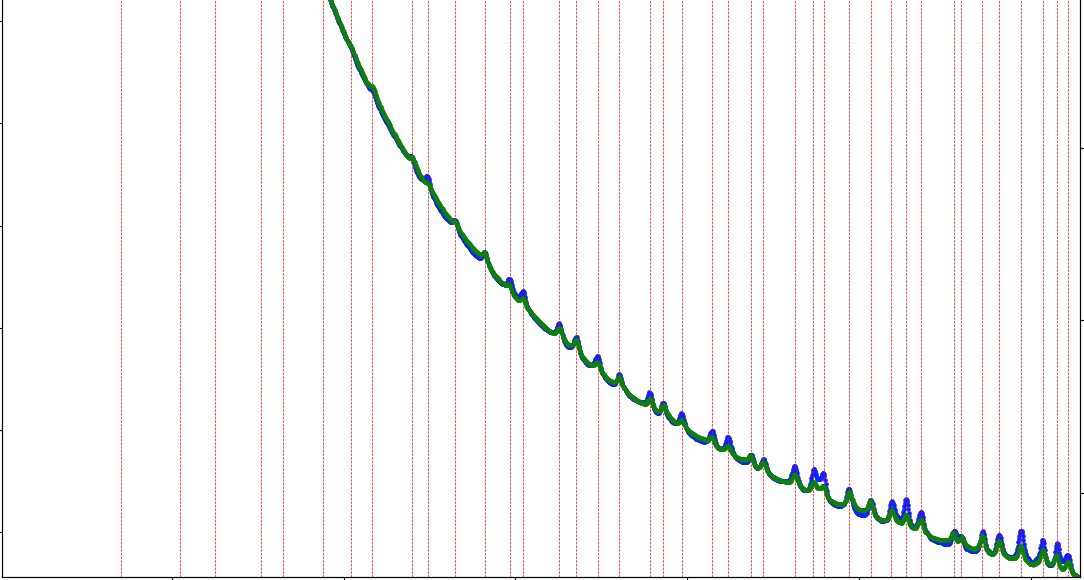
\includegraphics[width=0.8\linewidth]{../images/zoomed_scattering.png}
   
\caption{Scattering amplitude for finite $L_{\chi}$. Vertical red lines indicate the positions of the imaginary part of the non-trivial zeros of the RZF.}
\label{default}
\end{center}
\end{figure}


\section{Conclusion}
\section{Acknowledgements}
I gratefully acknowledge helpful conversations with CY Fong, John Baez, Jamison Galloway, Robert Hayre, Chun Yen Lin and Catalin Spataru.
\section{Appendix}



\end{document}  

